\documentclass{beamer}
\title[Elicitation and Explanation in Social Choice]{Elicitation and Explanation in Social Choice Theory}
%\subtitle{Proposal: ``Elicitation and Explanation for Voting Rules''}
\author{Beatrice Napolitano}
\date{18 December 2018}


\usetheme{CambridgeUS}
\usecolortheme{beaver}

\usepackage{tikz}
\usepackage{amsmath}
\usepackage{graphicx}
\newcommand{\ppref}{\succ^\text{p}}

\definecolor{darkred}{rgb}{0.8,0,0}

\begin{document}

\beamertemplatenavigationsymbolsempty

\begin{frame}[plain]
\maketitle
\end{frame}

\addtocounter{framenumber}{-1}

%\section*{Outline}
%\begin{frame}
%\tableofcontents
%\end{frame}

%\section{Education and Experience}
%\begin{frame}
%\frametitle{Education and Experience}
%\begin{block}{Education}
%	\begin{itemize}
%		\item \textbf{2014-ongoing} Master's Degree in Computer Engineering, University of Calabria (\textit{GPA 28.7/30}) 
%		\item \textbf{2011-2014} Bachelor's Degree in Computer Engineering, University of Calabria, with highest grade (\textit{110/110})
%	\end{itemize}
%\end{block}
%\begin{alertblock}{Teaching Experience}
%	\begin{itemize}
%		\item \textbf{2015-2016} Academic Tutor for undergraduate courses:
%		\begin{itemize}
%			\item Graphical User Interfaces and Event-Driven Programming
%			\item Fundamentals of Informatics
%		\end{itemize}
%	\end{itemize}
%\end{alertblock}
%\end{frame}
%
%\begin{frame}
%\begin{block}{International Experience}
%	\begin{itemize}
%		\item \textbf{2017} Visiting Student, Universit\'e Toulouse I Capitole \textit{(France)}
%		\begin{itemize}
%			\item research activity (master's thesis)
%		\end{itemize}
%		\item \textbf{2015} Full Time Exchange Student, University of Rhode Island \textit{(USA)}, 30 ECTS, GPA 3.06/4
%		\begin{itemize}
%			\item one of the six MoSt scholarship recipients for Engineering Department
%		\end{itemize}
%		\item \textbf{2013} Full Time Exchange Student under ERASMUS programme, Warsaw University of Technology \textit{(Poland)}, 30 ECTS, GPA 4.5/5
%	\end{itemize}
%\end{block}
%\begin{alertblock}{Summer School}
%	\begin{itemize}
%		\item \textbf{2017} Participation to the 19th European Agent Systems Summer School \textit{EASSS'17}, University of Gda\'nsk \textit{(Poland)}
%	\end{itemize}
%\end{alertblock}
%\end{frame}
%
%\section{Master's thesis}
%%title, supervisors, field, related research, keywords
%\subsection*{Overview}
%\begin{frame}
%\frametitle{Master's Thesis}
%	{\color{darkred}\text{Title}:} Finding consensus over graph knowledge bases
%	\newline {\color{darkred}\text{Supervisors}:} Gianluigi Greco, Umberto Grandi
%	\newline {\color{darkred}\text{Graduation Date}:} 16-20 July 2018
%\begin{block}{}
%\textbf{Related work}: Graph aggregation, Endriss \& Grandi, 2017
%\newline \textbf{Goal}: Find an aggregation rule for a set of graphs that preserves certain properties of the single graphs
%\end{block}
%\begin{block}{}
%	{\color{darkred}\textbf{Idea}:} Find an aggregation for a set of graphs such that the collective graph satisfies certain properties
%	
%%	Given some properties:
%%	\begin{itemize}
%%		\item find an aggregation for a set of graphs such that the collective graph satisfies them
%%		\item quantify the changes that have to be done to the set of graphs in order to find such a collective graph if it does not exist
%%	\end{itemize}
%\end{block}
%\end{frame}
%
%\subsection*{Example}
%\begin{frame}
%\frametitle{An Example of Property}
%	\begin{figure}[h] 
%	\begin{tikzpicture}[ scale=1,
%	block/.style={
%		draw,
%		circle,
%		align=center,
%		font=\scriptsize}]
%	
%	\node[block, label={[magenta]below:{\scriptsize wellness}}]		(2) at (-6.5,7.4) {2};
%	\node[block, label={[orange]below:{\scriptsize politics}}]		(3) at (-8.8,6.5) {3};
%	\node[block, label={[red]below:{\scriptsize \{science, fitness\} }}] 		(4) at (-7.2,5.9) {4};
%	\node[block, label={[blue]below:{\scriptsize sport}}] 		(5) at (-5.3,6) {5};
%	\node[block, label={[cyan]below:{\scriptsize finance}}] 		(6) at (-8.8,4.7) {6};
%	
%	\draw [->] (4) edge (2);
%	\draw [->] (3) edge (4);
%	\draw [->] (4) edge (6);
%	\draw [->] (6) edge (3);
%	\draw [->] (4) edge (5);
%	
%	\end{tikzpicture}
%\end{figure}
%	Every node labeled \textit{finance} follows a node labeled \textit{politics}
%\begin{equation*} 
%\tau = ((\text{finance}) \times (\text{politics}))  \sqsubseteq (\text{finance}\cdot \text{politics})
%\end{equation*}
%\end{frame}
%
%\subsection*{Setting}
%\begin{frame}
%\frametitle{Setting}
%	\begin{description}[$G=\langle N,E,\lambda \rangle$]
%		\item [$\Sigma$] the label alphabet
%		\item [$\Upsilon$] the nodes alphabet
%		\item [$G=\langle N,E,\lambda \rangle$] denotes a \emph{graph}, with
%		\begin{description}
%			\item [$N\subseteq \Upsilon$] the set of nodes
%			\item [$E\subseteq N\times N$] the set of oriented edges
%			\item [$\lambda:N \rightarrow 2^\Sigma$] the labeling function
%		\end{description}
%	\end{description}
%\end{frame}
%
%\subsection*{Formulas}
%\begin{frame}
%\frametitle{Formulas}
%
%	We defined a logical language $\mathcal{L}$
%	\begin{description}[$ \tau ::= \ \phi_1 \sqsubseteq \phi_2 $]
%		\item [$ \tau ::= \ \phi_1 \sqsubseteq \phi_2 $] a formula of the language $\mathcal{L}$
%		\item [$G \models \tau$] if $G$ is a model of $\tau$
%	\end{description}
%
%\begin{exampleblock}{Example of a more complicated formula}
%\footnotesize{\begin{multline*}
%	\tau_2 = ( \ (\text{science})\times (\text{finance}))_{|_s} \cup ((\text{science})\times (\text{politics}))_{|_s} \ ) \sqsubseteq \\ ( \ (\text{science} \cdot (( \text{finance $\cdot$ politics}) + ( \text{politics $\cdot$ finance}  )) \cdot \text{science})_{|_s} \ ) 
%	\end{multline*}}
%\end{exampleblock}
%\end{frame}
%
%\subsection*{Result}
%\begin{frame}
%\frametitle{First Result}
%{\color{darkred} $\tau$-model checking is polynomial in the size of the input}
%
%	\medskip
%
%	\begin{tabular}{|r|l|}
%		\hline
%		% after \\: \hline or \cline{col1-col2} \cline{col3-col4} ...
%		Name: &  \textrm{$\tau$-model checking}		  	\\
%		Instance: & $G$, $\tau\in \mathcal{L}$     \\
%		Question: & Is $G$ a model of $\tau$ ?  \\
%		\hline
%	\end{tabular}
%
%\end{frame}
%
%\subsection*{Extensions}
%\begin{frame}
%\frametitle{Multiple Formulas}
%
%	\begin{description}[$\sigma=(\sigma_T,\sigma_F)$]
%		\item [$\sigma_T$] the set of formulas we want to be true
%		\item [$\sigma_F$] the set of formulas we want to be false
%		\item [$\sigma=(\sigma_T,\sigma_F)$] an interpretation of formulas
%	\end{description}
%\begin{block}{}
%A graph $G$ is a $\sigma$-\emph{model} if it satisfies the formulas in $\sigma_T$ and it doesn't satisfy the formulas in $\sigma_F$
%\end{block}
%%\begin{alertblock}{$\sigma$-model existence is NP-complete}
%	{\color{darkred} $\sigma$-model existence is NP-complete}
%	
%	\medskip
%	
%	\begin{tabular}{|r|l|}
%		\hline
%		% after \\: \hline or \cline{col1-col2} \cline{col3-col4} ...
%		Name: &  \textrm{$\sigma$-model existence}  \\
%		Instance: & $\sigma$       \\
%		Question: & Does there exist a $\sigma$-model?  \\
%		\hline
%	\end{tabular}
%
%
%\end{frame}
%
%\begin{frame}
%\frametitle{Multiple Graphs}
%
%	\begin{description}
%		\item [$\mathbf{G}$] the \emph{scenario}: a set of graphs defined over the same set of nodes
%		\item [$\Delta$] a distance defined over the graphs
%	\end{description}
%
%\begin{alertblock}{}
%	\begin{itemize}
%		\item A graph $G$ is a $\sigma$-\emph{consensus} graph for $\mathbf{G}$ if $G$ is the $\sigma$-\emph{model} that is the closest to the graphs in the scenario on average
%		\item In some cases no $\sigma$-\emph{model} exists
%		\item An interpretation $\sigma^*$ is a $\sigma$-\emph{repair} if $\sigma^*$ is the closest interpretation to $\sigma$ for which a $\sigma^*$-\emph{model} exists
%	\end{itemize}
%\end{alertblock}
%
%\end{frame}


\section{Ph.D. Proposal}
\subsection*{Goal}
\begin{frame}
\frametitle{Goal}
Develop procedures able to help a committee (or a society) choose a suitable voting rule
\newline \newline \textbf{Involves}:
\begin{itemize}
	\item Axiomatic analysis of voting rules
	\item Explanation of axioms in non-expert terms
	\item Preference elicitation methods
\end{itemize}
\end{frame}

\subsection*{Approach}
\begin{frame}
\frametitle{Approach}
	\textbf{Idea}: Automatically find properties which are incompatible  \newline \newline
	The inconsistencies proofs should be translated to non-expert terms and used for:
	\begin{itemize}
		\item querying the user and infer her preferences depending on her answers
		\item showing the user that she cannot have everything
		\item validate whether some choices are ``better'' than others
	\end{itemize}~\\	
	\textbf{More generally}: Work on elicitation procedures related to social choice
\end{frame}

\section{Current Work}
\subsection{Minimax Regret}

\begin{frame}
\frametitle{Robust Winner Determination}
	\textbf{Setting}: Two kind of players
\begin{figure}
	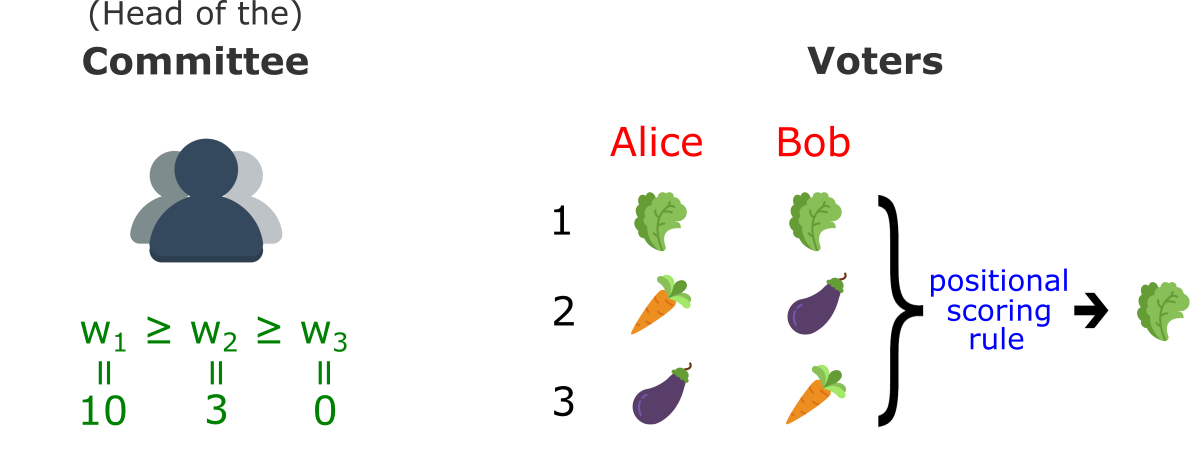
\includegraphics[scale=0.38]{setting.png}
	%		\caption{.}
	%		\label{fig:b1}
\end{figure}~\vspace*{15px}
\end{frame}

\begin{frame}
	\frametitle{Partial Knowledge}
	\textbf{Setting}: Incomplete profile and uncertain scoring rule
	\begin{figure}
		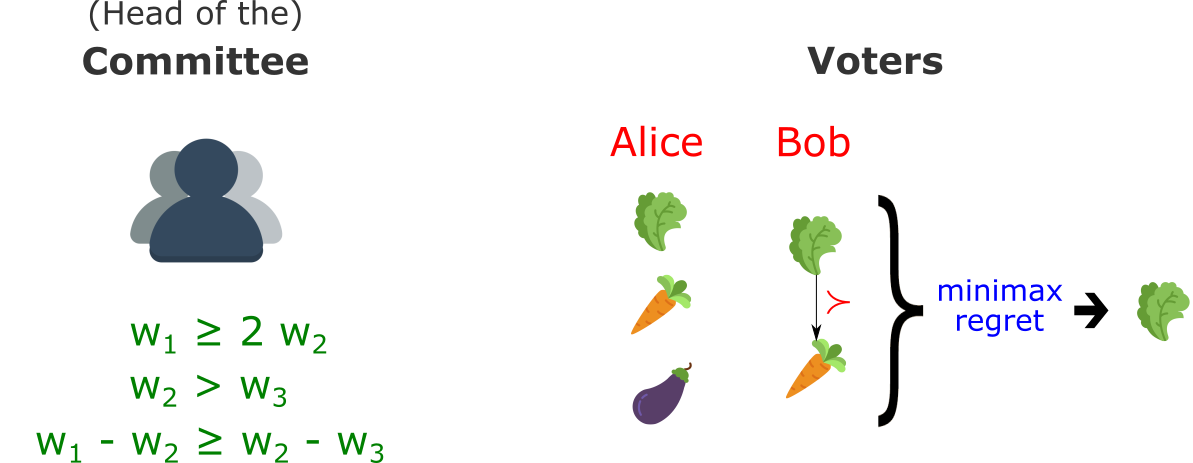
\includegraphics[scale=0.38]{setting2.png}
%		\caption{.}
%		\label{fig:b1}
	\end{figure}
	\textbf{Goal}: Winner determination using an incremental elicitation protocol based on minimax regret
\end{frame}

%\begin{frame}
%	\frametitle{Questioning strategy}
%	\begin{description} [$C(\textbf{p})=C(\ppref_1)\times \ldots \times C(\ppref_n)$]
%		\item[$A=\{a_1, \dots, a_m\}$] alternatives
%		\item [$N=\{1, \dots, n\}$] voters
%		\item [$w=(w_1, \dots, w_m)$] \textit{convex} scoring vector  
%		\item [$\ppref_i$] partial preference order of voter $i$
%		\item [$\textbf{p}=(\ppref_1,\ldots,\ppref_n)$] incomplete profile
%		\item [$C(\ppref_i)$] set of all complete rankings that extend $\ppref_i$
%		\item [$C(\textbf{p})=C(\ppref_1)\times \ldots \times C(\ppref_n)$] set of complete profiles extending $p$
%	\end{description}~\\
%	\textbf{Goal}: Winner determination using an incremental elicitation protocol based on minimax regret
%\end{frame}

\begin{frame}
	\frametitle{Max Regret}
		\begin{description} [$W=\{\mathbf{w}|\mathbf{w}=(w_1, \dots, w_m)\}$]
			\item [$A=\{a_1, \dots, a_m\}$] alternatives
			\item [$N=\{1, \dots, n\}$] voters
			\item [$V=\{\mathbf{v}|\mathbf{v}=(v_1, \dots, v_n)\}$] set of complete preference profiles
			\item [$W=\{\mathbf{w}|\mathbf{w}=(w_1, \dots, w_m)\}$] set of scoring vectors
			\item [$s(a;\mathbf{v},\mathbf{w})=\sum_{i \in N} \mathbf{w}_{\mathbf{v}_i(a)}$] score of the alternative \textit{a} under the profile \textbf{v} and weights \textbf{w}
		\end{description}~\\
	\begin{itemize}
		\item $\mathbf{\textbf{PMR}(a,b)}=\max_{\mathbf{w} \in W} \max_{\mathbf{v} \in V} s(b; \mathbf{v},\mathbf{w}) - s(a; \mathbf{v},\mathbf{w})$ 
		\item $\mathbf{\textbf{MR}(a)} = \max_{b \in A} \text{PMR}(a,b)$
	\end{itemize} 
	\begin{block}{}
		The winner is the alternative with minimal MR
	\end{block}
\end{frame}

\begin{frame}
\frametitle{Profile Completion}
\begin{figure}
	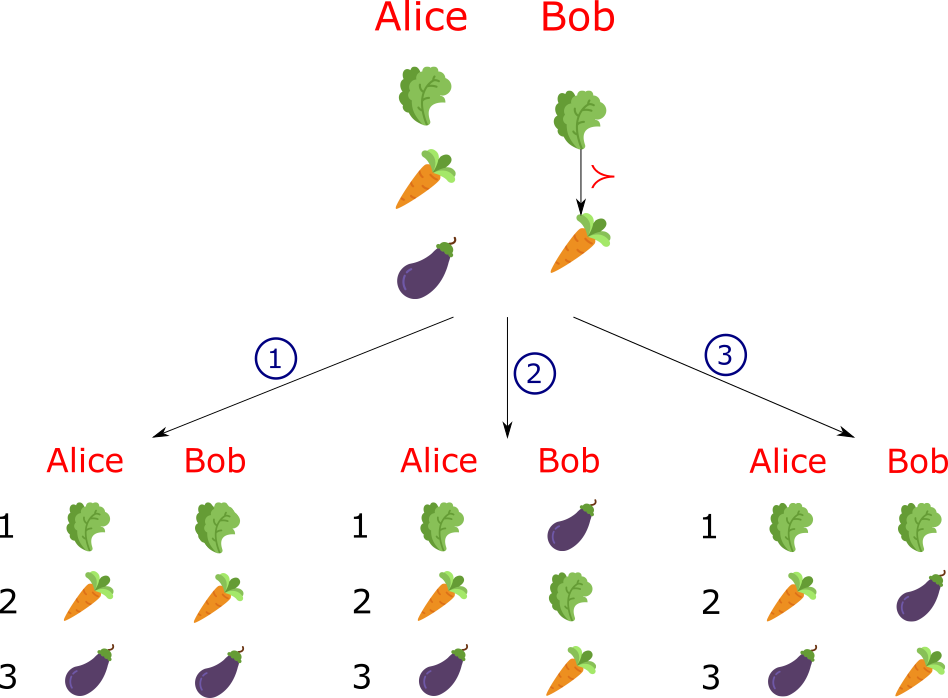
\includegraphics[scale=0.38]{completion.png}
	%		\caption{.}
	%		\label{fig:b1}
\end{figure}
\end{frame}

\begin{frame}
	\frametitle{Computing Minimax Regret}
		Admissible scoring vectors: $W=\{\mathbf{w}| \ w_1=10, \ 0 < w_2 \leq 5, \ w_3=0\}$~\vspace*{10px}
		\begin{figure}
			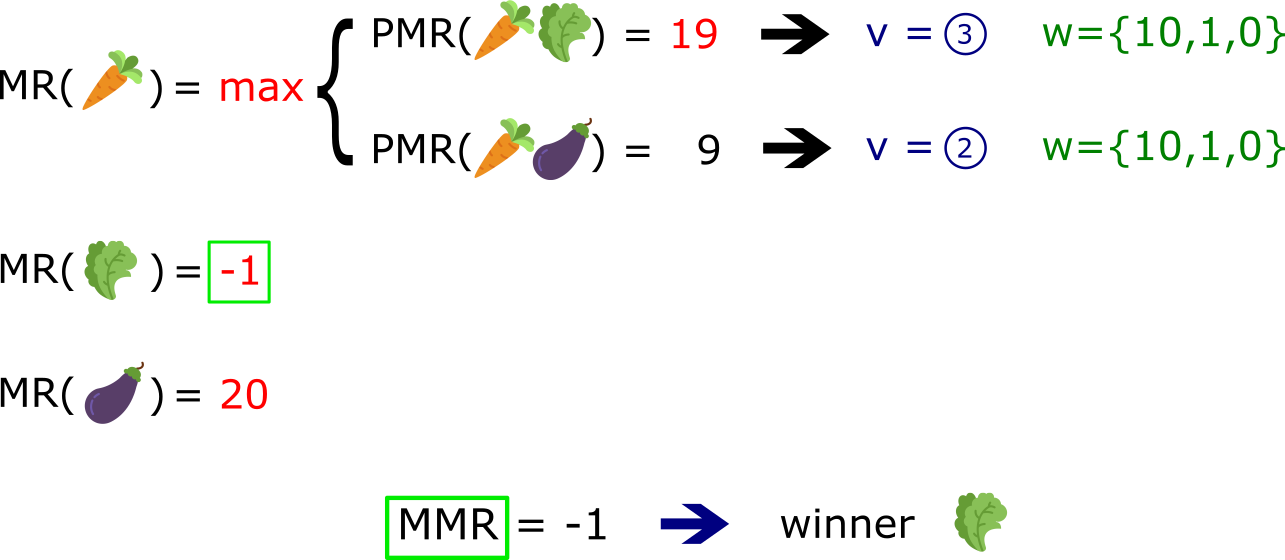
\includegraphics[scale=0.32]{comp.png}
			%		\caption{.}
			%		\label{fig:b1}
		\end{figure}
\end{frame}

\subsection{Related Works}
\begin{frame}
	\frametitle{Related Works}
	\textbf{Incomplete profile}  
	\begin{itemize}
		\item and known weights: Minimax regret to produce a robust winner approximation (\textit{Lu and Boutilier 2011}, \cite{Lu2011}; \textit{Boutilier et al. 2006}, \cite{Boutilier2006})
	\end{itemize}~\\
	\textbf{Uncertain weights} 
	\begin{itemize}
		\item and complete profile: dominance relations derived to eliminate alternatives always less preferred than others (\textit{Stein et al. 1994}, \cite{Stein1994})
		\item in positional scoring rules (\textit{Viappiani 2018}, \cite{Viappiani2018})
	\end{itemize}
\end{frame}

\addtocounter{framenumber}{-1}
\begin{frame}[plain]
	\centering \color{darkred}\LARGE Thank You!
\end{frame}




\bibliographystyle{plain}
\bibliography{biblio} 
%given a combination of axioms we want to find an outcome that doesn't satisfy them, and we would do that for several reasons:
%-querying the user, depending of her answer we might infer her preferences over the set of axioms;
%-proving that a set of axioms is not valid giving a counter-example;


%A method for automatically proving impossibility theorems in the area of ranking sets of objects has already been implemented (Geist \& Endriss, 2011). It:



\end{document}